%%%%%%%%%%%%%%%%%%%%%%%%%%%%%%%%%%%%%%%%%
% Short Sectioned Assignment
% LaTeX Template
% Version 1.0 (5/5/12)
%
% This template has been downloaded from:
% http://www.LaTeXTemplates.com
%
% Original author:
% Frits Wenneker (http://www.howtotex.com)
%
% License:
% CC BY-NC-SA 3.0 (http://creativecommons.org/licenses/by-nc-sa/3.0/)
%
%%%%%%%%%%%%%%%%%%%%%%%%%%%%%%%%%%%%%%%%%

%----------------------------------------------------------------------------------------
%	PACKAGES AND OTHER DOCUMENT CONFIGURATIONS
%----------------------------------------------------------------------------------------

\documentclass[paper=a4, fontsize=11pt]{scrartcl} % A4 paper and 11pt font size

\usepackage[T1]{fontenc} % Use 8-bit encoding that has 256 glyphs
\usepackage{fourier} % Use the Adobe Utopia font for the document - comment this line to return to the LaTeX default
\usepackage[english]{babel} % English language/hyphenation
\usepackage{amsmath,amsfonts,amsthm} % Math packages
\usepackage{url}

\usepackage{graphicx}
\usepackage{hyperref}
\usepackage{subfigure}
\usepackage{lipsum} % Used for inserting dummy 'Lorem ipsum' text into the template

\usepackage{sectsty} % Allows customizing section commands
\allsectionsfont{\centering \normalfont\scshape} % Make all sections centered, the default font and small caps

\usepackage{fancyhdr} % Custom headers and footers
\pagestyle{fancyplain} % Makes all pages in the document conform to the custom headers and footers
\fancyhead{} % No page header - if you want one, create it in the same way as the footers below
\fancyfoot[L]{} % Empty left footer
\fancyfoot[C]{} % Empty center footer
\fancyfoot[R]{\thepage} % Page numbering for right footer
\renewcommand{\headrulewidth}{0pt} % Remove header underlines
\renewcommand{\footrulewidth}{0pt} % Remove footer underlines
\setlength{\headheight}{13.6pt} % Customize the height of the header

\numberwithin{equation}{section} % Number equations within sections (i.e. 1.1, 1.2, 2.1, 2.2 instead of 1, 2, 3, 4)
\numberwithin{figure}{section} % Number figures within sections (i.e. 1.1, 1.2, 2.1, 2.2 instead of 1, 2, 3, 4)
\numberwithin{table}{section} % Number tables within sections (i.e. 1.1, 1.2, 2.1, 2.2 instead of 1, 2, 3, 4)

\setlength\parindent{0pt} % Removes all indentation from paragraphs - comment this line for an assignment with lots of text

%----------------------------------------------------------------------------------------
%	TITLE SECTION
%----------------------------------------------------------------------------------------
\newcommand{\itl}{\textit}
\newcommand{\horrule}[1]{\rule{\linewidth}{#1}} % Create horizontal rule command with 1 argument of height

\title{	
\normalfont \normalsize 
\textsc{University of Bucharest, College of Mathematics and Computer Science  } \\ [25pt] % Your university, school and/or department name(s)
\horrule{0.5pt} \\[0.4cm] % Thin top horizontal rule
\huge Sex beyond the genitalia,\\ The human brain mosaic 
 % The assignment title
\horrule{2pt} \\[0.5cm] % Thick bottom horizontal rule
}
\subtitle{-paper resume-}

\author{\c Stefan Cobeli} % Your name

\date{\normalsize\today} % Today's date or a custom date

\begin{document}

\maketitle % Print the title

%----------------------------------------------------------------------------------------
%	PROBLEM 1
%----------------------------------------------------------------------------------------

\section{Main idea}
\paragraph{}

	The authors of the present paper, lead by Daphna Joel, used magnetic resonance\\ imaging (MRI, method to analyze the human brain) on multiple samples of people.\\ They compared the results of the distribution of grey and white matter, internal consistency and other similar traits in the brain. The conclusion was that there exists extensive overlap between the distributions of the parameters, from person to person. 

\section{Contrary Opinions}
	\paragraph{}
		Over the time there was a long debate about differences between genders, that gave birth to a lot of myths, jokes and even conflicts in society. 
		For example, a stand-up comedian, Mark Gungor, used this subject in one of his sketches. He developed a theory which says that men have the brain structured in multiple different boxes and when they make a certain activity, they enter in the box that is specific to it and it's very hard to get out of there. Also men have a special box, the "nothing box", in which they enter if they are tired and don't have the mood of doing anything. This box is the most annoying for women, because they don't understand how can something like this exists. Gungor says that women brains are completely different because of the fact that they have only one box in which everything is interconnected and for this reason they have the ability to do everything in the same time.\\
		(Here is a link to the sketch \cite{NthB})
				
		\begin{figure}[h!]
			\centering
			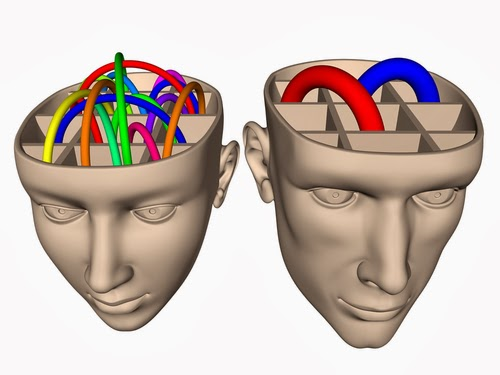
\includegraphics[scale=0.5]	{connectionesCerebrales.jpg}
		 	\caption{Women vs Men cartoon.}
 		
  			\label{fig:boat1}
  			
		\end{figure}

	\newpage\paragraph{}
		Returning to more serious matters, in a TV show ("The Agenda" at tvo television), \\Jordan Peterson, professor at Toronto University, argued against the hypothesis of\\ Daphna Joel and said that the gender differences in brain are present in our life from the first day. He invoked a study made on one day old children, in which it was discovered that little boys don't react to human faces as much as little girls do. Instead they are more attracted to the moving objects. This behavior may be favored by prenatal testosterone that is induced in the mother's womb especially to boys.\subparagraph{}
		Another idea in the show, launched by Daphna Joel, was that the  males and females should not be treated differently and such a behavior is the same with racism thinking between black and white people. At this idea, Jordan Peterson, said that we should acknowledge  those\\ dissimilarities because even between black and white people there are biological mismatches and it is important to all of us to know and understand them, so we can take advantage of every single difference and make it count in a good way (A similar case stands for racial differences. They exist and influence our body and it's important to know them, rather then treat everyone like those "little details" does not exist).\\
		(Other interesting details about this argue you can see in the full show \cite{TheAgenda}. Also we recommend you to watch "The Gender Equality Paradox" \cite{GEP}, a short documentary about how\\ people react in the most gender free society and the fact that when people are free to choose their path in life, they almost every time choose a job specific to their gender traditional jobs).		
			\newpage
\section{About the research field}\paragraph{}
	The idea that the male brain and female brain have no fundamental difference belongs to professor Daphna Joel from Tel-Aviv University and she published many articles on this direction. 
	She started to embrace this idea when she saw a study about the fact that the\\ hippocampus of man can change in 15 minutes to something that looks pretty much the same with the female one and the process is reciprocal. The stimulus that leads to this change is the presence of stress.\\
	
	
\begin{figure}[h!]
  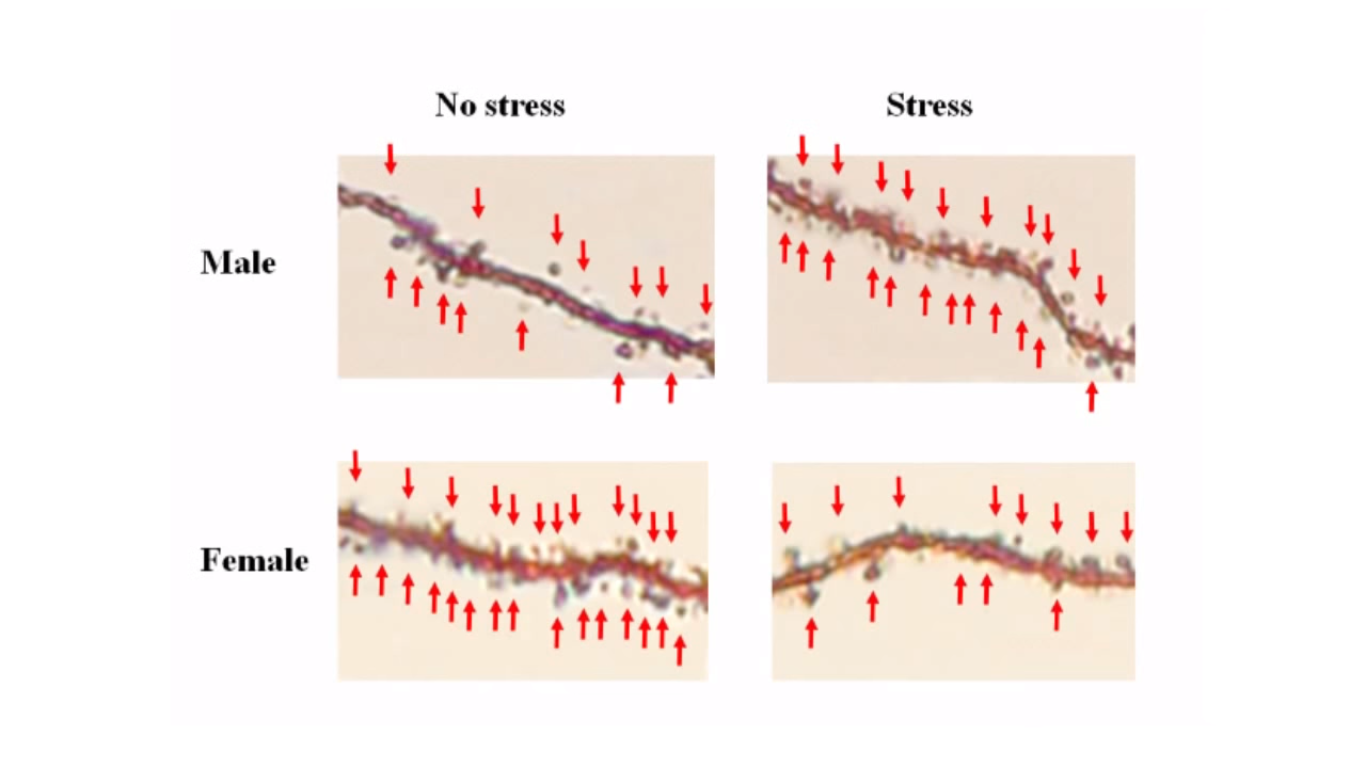
\includegraphics[width=\linewidth]{stressVSnoStressHippocampus.png}
 	\caption{Changing of Hippocampus in presence of stress.}
 	More details about this idea was presented by Daphna Joel in a Ted conference \cite{TED}.
  \label{fig:boat1}
\end{figure}

%%%%	You can see some of them in bibliography.\\


\newpage
	\section{Current paper}
		
		
		
		
			\subsection{Motivation}							\paragraph{}
The problem of classifying the human brains in male brains and female brains is still\\ unresolved, but it is widely spread the idea that those classes are disjoint.
Due to the fact that the prejudices affect some women and it is believed that their careers are hindered to develop, this paper comes with an argue that those ideas are ungrounded  and women can make men jobs and vice-versa.
The study comes as a continuation of a series of articles on this topic. Until now it was analyzed the attitude, interests, behavior and other similar traits and now this study comes with an examination of MRI's results on more than 1,400 human brains and conclude that the similarities are predominant.
\subsection{Significance}\paragraph{}
Differences between males and females were always present in the mind of humans.\\ Because of that, some could justify a differential treatment of males and females.
The present paper propose a new perception. Despite the fact that exists some gender differences in behaviour, we cannot divide the brains in two categories (i.e. male brain/female brain), but we can say that every brain is a unic mosaic of male/female common characteristics.


\begin{figure}[h!]
			\centering
			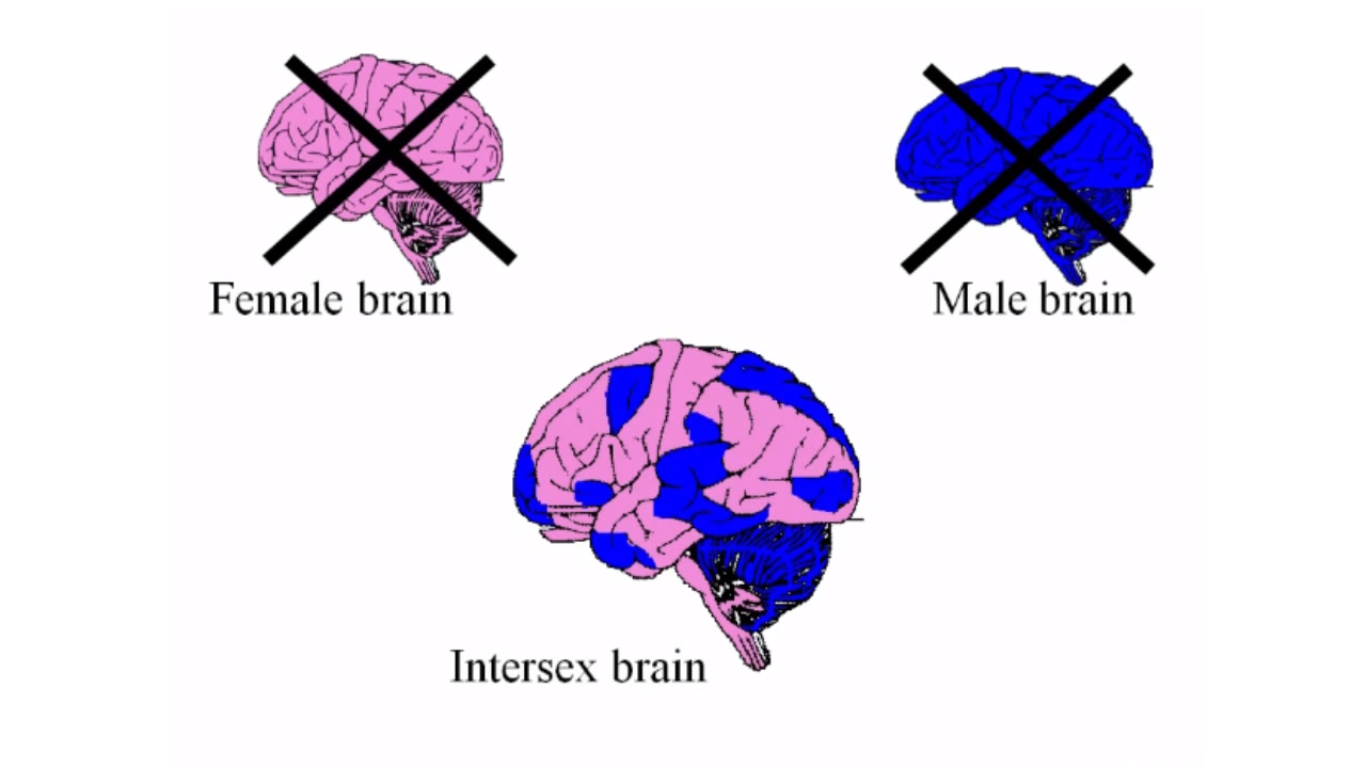
\includegraphics[scale=0.25]	{brainMosaic2.png}
		 	\caption{Vision of the authors about brains.}
 		
  			\label{fig:ends}
  			
		\end{figure}


\subsection{Principal results}
	\paragraph{}
			In the picture from above it is suggested that the brain doesn't have a certain consistency depending on its sex, rather every brain has its own components of both male and female predominant features.
			There was defined the notions of \itl{"female-end"} and \itl{"male-end"} that means the 33\% most common results of females and males respectively, so this notions refer at the characteristics that are mostly prevalent in one of the genders (you can see a representations of this concept above, in Figure \ref{fig:ends}, where the \itl{female-end} features are coloured in pink and the \itl{male-end} features are coloured in blue).\paragraph{}
	The present paper compares the internal consistency degree of multiple samples of brains with several different imaging modalities and analyse them with multiple methods to increase the chance that the results are not dependent of measure, analyse methods, samples etc.
	The research was focused on the brain regions that showed larger sex differences until now (e.g. the hippocampus or the caudate) and the results showed that even on these regions there exists lots of similarities.\\
	The results of analysing the samples showed that most people have both "\itl{female-end}" and "\itl{male-end}" characteristics, rather then have an internal consistency at one of those ends.
	\hrule\hrule\hrule\paragraph{}
Further the reader can analyse the most important results of this article structured in the table below, where every line represents a different sample of people that participated to this study.
		\begin{figure}[h!]
			\centering
			\includegraphics[scale=0.82]	{table1.png}
 		
  			\label{fig:table}
  			
		\end{figure}
		
		\newpage
		
		
	\paragraph{Little review about how the measurements were made}
	
		After assessing the brains on gray matter volume (this is represented in Figure \ref{fig:graphics} A and B. The evaluation was made using voxel-based morphometry(VBM))  first ten regions that showed the largest difference between sexes were selected to make a more detailed research \\(the regions compared were defined using Automated Anatomical Labeling atlas(AAL) \cite{AAL}. This regions are illustrated in Figure \ref{fig:graphics} C).		
		
		
		\begin{figure}[h!]
			\centering
			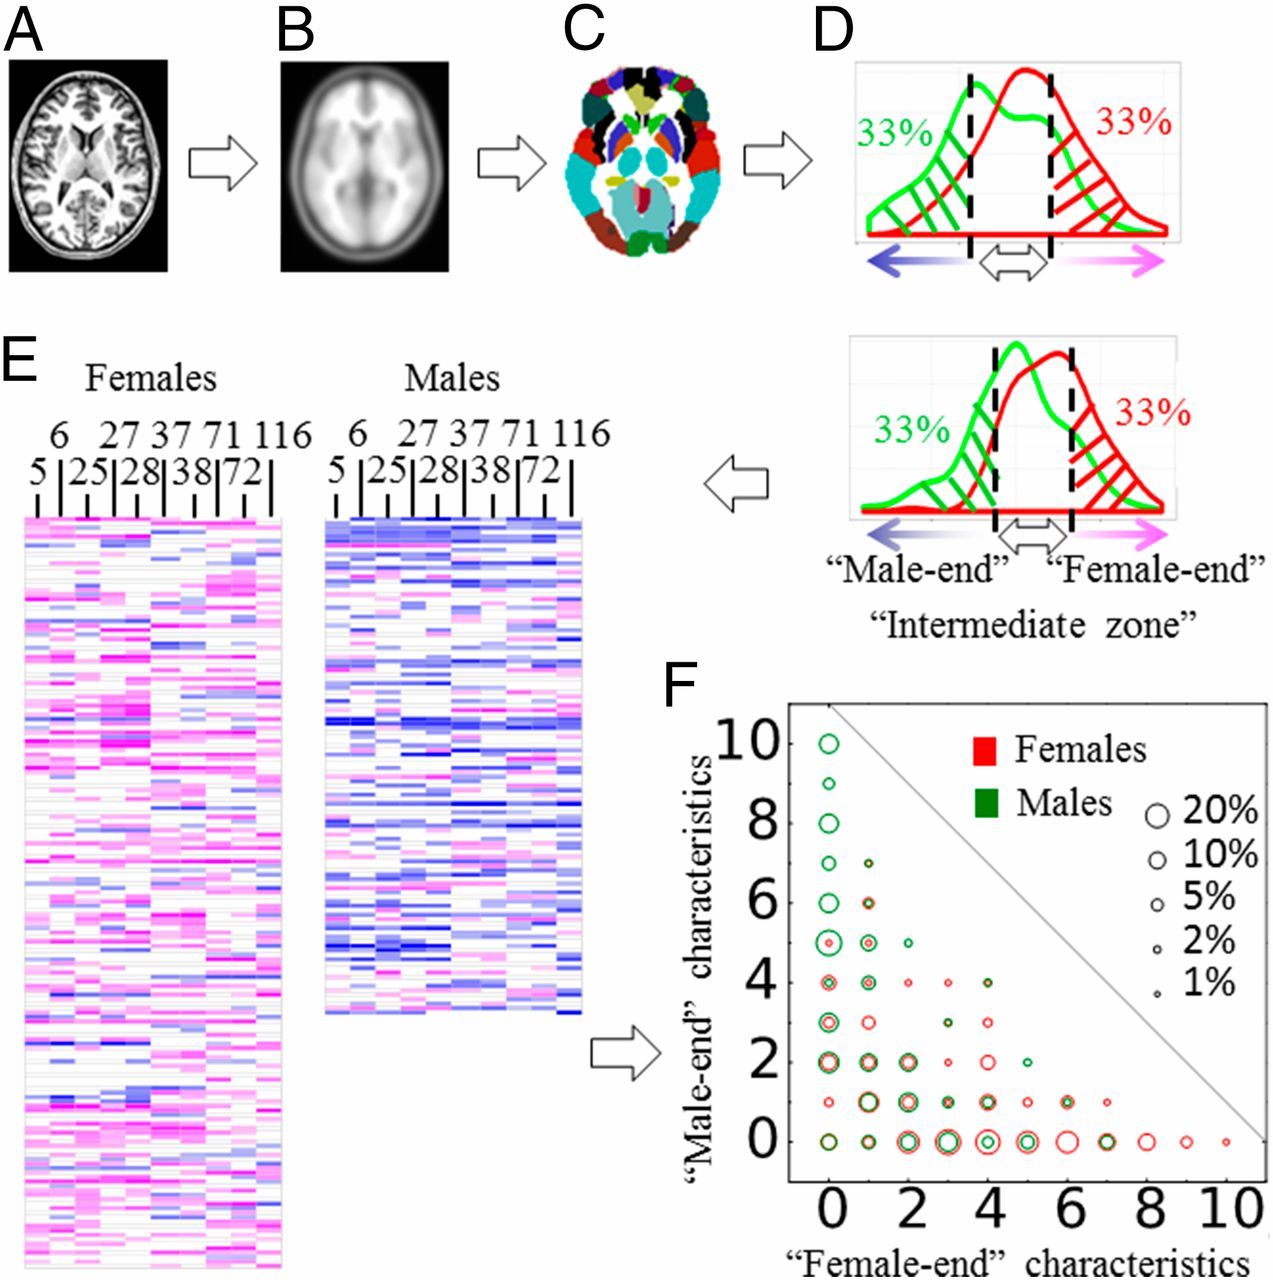
\includegraphics[scale=0.82]	{paperGraphics.jpg}
			\caption{The path of brain evaluation, in this study. }
 		
  			\label{fig:graphics}
  			
		\end{figure}
		\paragraph{}
		Figure \ref{fig:graphics} D shows the distributions of the gray matter volume in two of the regions that were previously selected for high difference, the left hippocampus (first picture) and the left caudate (second picture). With green color is represented the males and with red color the females. For each of the principal ten regions were made such graphics.
		The last two pictures from Figure \ref{fig:graphics}, E and F presents  the same result but in different ways. In the first one you can see two strips. Both are divided in 116 columns, each corresponding to a brain region from the AAL atlas \cite{AAL} and both have multiples rows, each corresponding to a subject. The left stripe represents the female subjects and the right one the male subjects.\\
		So we can visualize those strips as two matrices.  You can observe that there are blue, pink and white cells. The blue ones correspond to regions of brain that are included in what \\the authors defined as "\itl{male-end}" and the pink ones correspond to regions from the\\ "\itl{female-end}", finally the white ones  are in neither of those classes, but the authors call them to be part of the "\itl{intermediate zone}". We can observe that very few of the lines have the same color, therefore most people have brain parts that have gray matter volume specific to their opposite sex in that specific part.
		The F picture is a bivariate scattergram for the same information presented above (it was create using the Matplotlib library from Python).
		\paragraph{}In Figure \ref{fig:graphics} was presented the assessment of a single dataset. Similar work was made for the other datasets and the results were alike(the reader shall see now with different eyes the table from Figure \ref{fig:table} with those new information gained).
		\paragraph{} 
		The authors claim that their result agrees well with studies (e.g. \cite{BONUS1}, \cite{BONUS2}) that demonstrates the possession of humans of both masculine and feminine psychological characteristics and that uni-dimensional
(masculinity-femininity) or a bi-dimensional (masculinity x femininity) model are outdated.
	
		
		

\subsection{Conclusions}\paragraph{}
The fact that the brain consistency presents such a variability from case to case,\\ independent of the gender differences, suggest that we should be more careful on\\ the uniqueness of each person and not only  to include it into a template of male or female. The authors consider that this idea can have a  big impact at social level and can cause public debates about single-sex education and gender as a social category.

\newpage
\lipsum[200] 

{\small
\begin{thebibliography}{9999}

\bibitem{MAIN} Joel D et al. 2015 Sex beyond the genitalia:
the human brain mosaic. Proc. Natl Acad. Sci. USA 

\bibitem{NthB} "The Nothing Box"\\
\url {https://www.youtube.com/watch?v=3XjUFYxSxDk}\\

\bibitem{TheAgenda} Argue between Daphna Joel and Jordan Peterson in the "The Agenda" tv show.\\ "Gender and the Brain"\\
\url{https://www.youtube.com/watch?v=sSIEs1ngNiU}

\bibitem{GEP} "The Gender Equality Paradox"\\
\url{https://www.youtube.com/watch?v=p5LRdW8xw70}

\bibitem{TED}"TEDxJaffa -- Daphna Joel -- Are brains male or female?"\\
\url{https://www.youtube.com/watch?v=rYpDU040yzc}

\bibitem{AAL} Tzourio-Mazoyer N, et al. (2002) Automated anatomical labeling of activations in
SPM using a macroscopic anatomical parcellation of the MNI MRI single-subject brain.

\bibitem{BONUS1} Lippa RA (2005) Gender, Nature, and Nurture (Psychology Press, New York), 2nd Ed.

\bibitem{BONUS2} Spence JT (1993) Gender-related traits and gender ideology: Evidence for a multifactorial
theory. J Pers Soc Psychol



\end{thebibliography}
}

%------------------------------------------------


%----------------------------------------------------------------------------------------

\end{document}